% This is samplepaper.tex, a sample chapter demonstrating the
% LLNCS macro package for Springer Computer Science proceedings;
% Version 2.20 of 2017/10/04
%
\documentclass[runningheads]{llncs}
%
\usepackage{graphicx}
% Used for displaying a sample figure. If possible, figure files should
% be included in EPS format.
%
% If you use the hyperref package, please uncomment the following line
% to display URLs in blue roman font according to Springer's eBook style:
% \renewcommand\UrlFont{\color{blue}\rmfamily}

\begin{document}
%
\title{Contribution Title\thanks{Supported by organization x.}}
%
%\titlerunning{Abbreviated paper title}
% If the paper title is too long for the running head, you can set
% an abbreviated paper title here
%
\author{First Author\inst{1}\orcidID{0000-1111-2222-3333} \and
Second Author\inst{2,3}\orcidID{1111-2222-3333-4444} \and
Third Author\inst{3}\orcidID{2222--3333-4444-5555}}
%
\authorrunning{F. Author et al.}
% First names are abbreviated in the running head.
% If there are more than two authors, 'et al.' is used.
%
\institute{Princeton University, Princeton NJ 08544, USA \and
Springer Heidelberg, Tiergartenstr. 17, 69121 Heidelberg, Germany
\email{lncs@springer.com}\\
\url{http://www.springer.com/gp/computer-science/lncs} \and
ABC Institute, Rupert-Karls-University Heidelberg, Heidelberg, Germany\\
\email{\{abc,lncs\}@uni-heidelberg.de}}
%
\maketitle              % typeset the header of the contribution
%
\begin{abstract}
The abstract should briefly summarize the contents of the paper in
15--250 words.

\keywords{First keyword  \and Second keyword \and Another keyword.}
\end{abstract}
%
%
%
\section{Health Section}
\subsection{Data Collection}
For the health section in this project, we want to show how COVID-19 changed the world in public health on three aspects: confirmed number of cases, deaths, and vaccinated number of persons. 
The related COVID-19’s data is collected from Johns Hopkins University(JHU) CSSE COVID-19 dataset \cite{JHU_url} and the dataset of Our World in Data(owid) on Github \cite{owid_url}. 
For the global COVID-19 confirmed cases and deaths, the data is collected from 2020 to 2021 year. The collected data of global vaccinated number of persons is from 2021 year.
Each country's location of the global maps in this section uses the spatial data of World Atlas TopoJSON. We used Python coding to filter some blank objects in each data.
And we adjusted the country's name from the map location data to let it matching the name from each COVID-19’s data.

\subsection{Approach and Design} 
When we visualize these collected data, we try to realize the data visualization with balancing the objectivity, functionality, precision, and beauty. We base on the design rule that the visualizing form follows function. The form of infographic we chosed is according to how to let our audiences to get what they would like to know from we designed d3 graphics as much as possible \cite{albertocairo2012ggplot2}.\\
For visualizing the collected data of global COVID-19 confirmed cases, we design an interactive d3 proportional symbol map. On each country area of this map, the users can directly see the bubble size of the confirmed cases is changing with the time when the user drags the time slider. 
On this way, the users can clearly and directly know the growth speed of COVID-19 confirmed cases in each country. The second d3 chart in this section of our project is an interactive bar chart, the users can easily compare each country as the total confirmed cases or total deaths by sorting in different dimensions, like sorting by ascending number of persons, sorting by alphabetical order of name or sorting by ascending GDP in 2020 year. 
Through this interactive bar chart, users can fastly know which country’s public health is gravely impacted by the coronavirus. The last map in this section is an interactive and responsive d3 global choropleth map with color scale that presents the global cumulative the number of people vaccinated. 
As the filled color darker green means there are more people are vaccinated in this area, users can intuitively understand the status of vaccinating in global. When the users can click the country area on the map, there appears a pie chart of the vaccination rate status and a line chart of the cumulative confirmed COVID-19 cases of the selected country on the right side of the map. By this way, users can know taking vaccination is a way to protect themselves, but only by vaccinating cannot fastly decrease the confirmed rate of COVID-19.
Both on these two COVID-19 global maps in this section, users also can fastly know the country’s name or with some information by mouse hovering. 

\begin{figure}
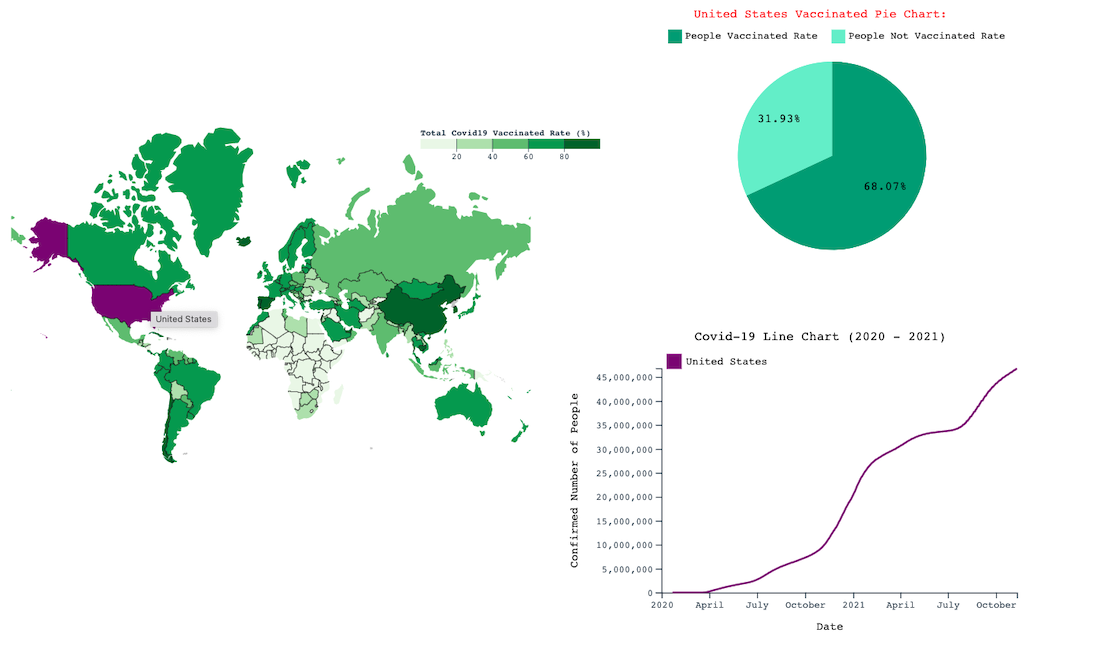
\includegraphics[width=\textwidth]{health3.png}
\caption{Selected United States on the D3 global choropleth map to respectively get the info of the vaccination rate status and the cumulative status of confirmed COVID-19 cases of this country by a pie chart and a line chart changing with time} \label{fig1}
\end{figure}

\bibliographystyle{splncs04}
\bibliography{references}

%
\end{document}
